\documentclass[bachelor, och, referat, times]{SCWorks}
% параметр - тип обучения - одно из значений:
%    spec     - специальность
%    bachelor - бакалавриат (по умолчанию)
%    master   - магистратура
% параметр - форма обучения - одно из значений:
%    och   - очное (по умолчанию)
%    zaoch - заочное
% параметр - тип работы - одно из значений:
%    referat    - реферат
%    coursework - курсовая работа (по умолчанию)
%    diploma    - дипломная работа
%    pract      - отчет по практике
%    pract      - отчет о научно-исследовательской работе
%    autoref    - автореферат выпускной работы
%    assignment - задание на выпускную квалификационную работу
%    review     - отзыв руководителя
%    critique   - рецензия на выпускную работу
% параметр - включение шрифта
%    times    - включение шрифта Times New Roman (если установлен)
%               по умолчанию выключен
\usepackage[T2A]{fontenc}
\usepackage[utf8]{inputenc}
\usepackage{graphicx}

\usepackage[sort,compress]{cite}
\usepackage{amsmath}
\usepackage{amssymb}
\usepackage{amsthm}
\usepackage{fancyvrb}
\usepackage{longtable}
\usepackage{array}
\usepackage[english,russian]{babel}
\usepackage{minted}
\usepackage{caption}
\usepackage{subcaption}
\setminted[python3]{fontsize=\small, breaklines=true, style=bw, linenos}
% Используется автором репозитория
%\usemintedstyle{xcode}
% Этот пакет включает в себя аналогичный Times New Roman шрифт.
% Необходим для успешной компиляции для UNIX-систем ввиду отсутствия TNR в нем.
% Можно использовать и для Windows.
%\usepackage{tempora}
\usepackage{tgtermes}


\usepackage[colorlinks=false]{hyperref}


\newcommand{\eqdef}{\stackrel {\rm def}{=}}
\renewcommand\theFancyVerbLine{\small\arabic{FancyVerbLine}}
\newtheorem{lem}{Лемма}

% % При использовании biblatex вместо bibtex
%\usepackage[style=gost-numeric]{biblatex}
%\addbibresource{thesis.bib}

\begin{document}

% Кафедра (в родительном падеже)
\chair{информатики и программирования}

% Тема работы
\title{Анализ социальных сетей}

% Курс
\course{1}

% Группа
\group{151}

% Факультет (в родительном падеже) (по умолчанию "факультета КНиИТ")
\department{факультета компьютерных наук и информационных технологий}

% Специальность/направление код - наименование
%\napravlenie{02.03.02 "--- Фундаментальная информатика и информационные технологии}
%\napravlenie{02.03.01 "--- Математическое обеспечение и администрирование информационных систем}
%\napravlenie{09.03.01 "--- Информатика и вычислительная техника}
\napravlenie{09.03.04 Программная инженерия}
%\napravlenie{10.05.01 "--- Компьютерная безопасность}

% Для студентки. Для работы студента следующая команда не нужна.
%\studenttitle{Студентки}

% Фамилия, имя, отчество в родительном падеже
\author{Янченко Вадима Александровича}

% Заведующий кафедрой
%\chtitle{доцент, к.\,ф.-м.\,н.} % степень, звание
%\chname{С.\,В.\,Миронов}

%Научный руководитель (для реферата преподаватель проверяющий работу)
%\satitle{доцент} %должность, степень, звание
%\saname{А.\,П.\,Грецова}

% Руководитель практики от организации (только для практики,
% для остальных типов работ не используется)
\patitle{к.\,ф.-м.\,н., доцент}
\paname{А.\,П.\,Грецова}

% Семестр (только для практики, для остальных
% типов работ не используется)
\term{2}

% Наименование практики (только для практики, для остальных
% типов работ не используется)
\practtype{учебная}

% Продолжительность практики (количество недель) (только для практики,
% для остальных типов работ не используется)
\duration{2}

% Даты начала и окончания практики (только для практики, для остальных
% типов работ не используется)
\practStart{01.07.2016}
\practFinish{14.07.2016}

% Год выполнения отчета
\date{2023}

\maketitle

% Включение нумерации рисунков, формул и таблиц по разделам
% (по умолчанию - нумерация сквозная)
% (допускается оба вида нумерации)
%\secNumbering


\tableofcontents

% Раздел "Обозначения и сокращения". Может отсутствовать в работе
% \abbreviations
% \begin{description}
%     \item ... "--- ...
%     \item ... "--- ...
% \end{description}

% Раздел "Определения". Может отсутствовать в работе
%\definitions

% Раздел "Определения, обозначения и сокращения". Может отсутствовать в работе.
% Если присутствует, то заменяет собой разделы "Обозначения и сокращения" и "Определения"
%\defabbr


% Раздел "Введение"

\intro
Сегодня каждый из нас использует социальные сети. Уже стало привычкой проверить утром публикации любимых сообществ, <<лайкнуть>> новое фото приятеля, переслать смешные картинки друзьям. Миллиарды людей ежедневно создают триллионы подобной информации. Социальные сети хранят все действия пользователей, а также многие социально"=демографические данные этих пользователей в открытом доступе. 

Современные программные средства позволяют собрать, проанализировать, визуализировать и получить вывод из собранных данных, которые сформированны миллионами сообщений, ссылок, постов, фотографий, и видео. Таким образом обнаруживаются связи между объектами, которые невозможно было бы получить без анализа социальных сетей. Изучение таких данных в определенных темах является одним из способов анализа тенденций изменения общественного
мнения в широком спектре вопросов, а результаты
анализа могут быть использованы в различных областях для решения задач практической направленности, включая задачи антитеррористической
направленности, прогнозирование потребности,
политические прогнозы, маркетинговые исследования, оценка репутационных рисков компании
или физического лица\cite{Tomsk_research}.

Цель данной работы "--- изучение основных методов анализа социальных сетей и применение их на практике.
% Целью данной работы является сбор и анализ данных подписчиков сообщества <<СГУ факультета КНиИТ>> \footnote{\url{https://vk.com/sgu_kniit}} и сообщества <<Душевно>>\footnote{\url{https://vk.com/somethinggoodforyoursoul}}.
% В ходе работы должны быть решены следующие задания:
% \begin{enumerate}
%     \item Изучение понятий социального графа
%     \item Изучение методов анализа социальных сетей, 
%     \item Сбор данных пользователей, подписанных на выбранные сообщества
%     \item Анализ полученного графа
% \end{enumerate}

% После введения — серии \section, \subsection и т.д.
\section{История возникновения социальных сетей}
Под социальной сетью понимается множество пользователей, которые могут выступать во взаимодействие друг с другом. С формальной точки зрения такие сети удобно представлять в виде графов и применять для анализа математические модели.

Впервые такой термин был введен в 1954 году социологом из <<Манчестерской школы>> Джеймсом Барнсом в работе <<Классы и собрания в норвежском островном приходе>>. В своей работе он охарактеризовал социальную сеть следующим образом: <<Каждый человек имеет определенный круг друзей, а эти друзья имеют, в свою очередь собственных друзей. Некоторые из друзей одного человека знают друг друга, а другие "--- нет. Я нашел удобным говорить о такого рода полях как о сетях. Под этим мне видится система точек, некоторые из которых соединины между собой. Точками этой системы являются люди а линии соединения этих точек указывают, какие люди взаимодействуют друг с другом>>\cite{Sazanov}.

Тема социального графа стала популярна после конференции Facebook F8 в 2007 году, на котором Марк Цукенберг представил программное обеспечение, которое собирает данные пользователей и взаимоотношения между ними\cite{CBSNews}.

Сегодня анализ социальных сетей является одним из наиболее популярных инструментов в мире бизнеса, маркетинга, политики и науки. Существует множество специализированных компаний, которые предоставляют подобные услуги. Они используют различные инструменты и методы для сбора и анализа данных из социальных сетей.
%Анализ социальных сетей имеет огромную ценность для бизнеса, так как позволяет понять ценность продукта для конкретной аудитории и как стоит его продвигать. Кроме того, анализ социальных сетей позволяет выдавать персонализированную рекламу, что имеет коммерческую выгоду для компаний. Социальными сетями пользуются опасные преступники, террористы для осуществление деструктивной деятельности. Анализ социальных сетей позволяет выявлять подобные группы и защищать обычных людей от их влияния\cite{hansen2010analyzing}.

\section{Основные определения в анализе социальных сетей}
\subsection{Метрики}
\textit{Метрики} "--- это числовые показатели, которые отображают характеристику объектов, сегментов, групп и их связей. Так как анализ социальных сетей чаще всего применяется в изучении человеческих взаимоотношений и взаимосвязей, то многие метрики пришли из социологии.

\textit{Гомофилия} "--- это степень, с которой индивид сформирует связь с схожим участником. Схожесть может быть определена по половому признаку, расе, возрасту и т.д. Эту концепцию лучше всего описывает пословица <<Рыбак рыбака видит из далека>>.

\textit{Соседство} "--- это склонность к появлению связей между индивидами по географическому признаку.

\textit{Обоюдность} или \textit{взаимность} "--- это степень, с которой у двух участников образуется двусторонняя связь\cite{kadushin2012understanding}.

\textit{Закрытость сети} "--- метрика полноты сети. Напрмер, закрытость сети говорит о том, сколько ваших друзей являются друзьями\cite{wong2014design}.

\textit{Мостом} называют связь, которая обеспечивает единственный путь между двумя вершинами. Например, мост между $A$ и $B$ означает, что путь информации от любого контака $A$ до любого контакта $B$ содержит эту связь\cite{Granovetter}.

\textit{Кликой} в теории графов определяют как подграф, в котором каждая пара вершин соединена ребром. В социологии же кликой называют группу людей, которые взаимодействуют друг с другом чаще и интенсивнее\cite{wong2014design}.

\subsection{Центральность}
Центральность это ещё одна метрика социального графа. Она определяет, насколько  <<важной>> является вершина в сети, основываясь на некоторых объективных критериях\cite{hansen2010analyzing}. Понятие <<важности>> узла можно определять по"=разному, поэтому существует несколько видов центральности, каждая из которых применима в определенной ситуации. Выделим несколько из них.

Одной из самых простых трактовок <<важности>> вершины является её степень, то есть количество входящих и выходящих из этой вершины ребер. Вычисление степеней каждой вершины в сети и сортировка их в порядке убывания даст ранг локальной (степенной) центральности. Эта центральность называется локальной, поскольку она выделяет точки, которые хорошо связаны между собой в непосредственной близости\cite{scott2012social}.

Можно подойти к вопросу <<важности>> вершины с другой стороны. Выделим вершины, которые ближе всего ко всем остальным. Степень близости узла вычисляется по формуле
\begin{equation*}
    C(v) = \frac{N}{\sum_u{d(v,u)}},
\end{equation*}
где $d(v,u)$ равно расстоянию между вершина $v$ и $u$, а $N$ "--- количество узлов. Близость применятеся в разных сферах. Так, в библиометрии степень близость показывает насколько в среднем близка одна дисциплина ко всем другим в сети\cite{bibliometrics}. В социальных сетях же установлено, что продвижение товара пользователям с наибольшей степенью близости ведёт к огромной выгоде\cite{closeness_marketing}.

Также существует другой вариант вычисления степени близости в неориентированном графе:
\begin{equation*}
    H(v) = \frac{1}{N - 1} \cdot  \sum_{u\vert u \neq v}{\frac{1}{d(u,v)}},
\end{equation*}
где $1/d(u,v) = 0$, если нет пути из $v$ в $u$, $N$ "--- количество узлов. Центральность, основанная на такой формуле, называется гармонической.

Кроме того, определение <<важной>> вершины можно дать через кратчайший путь. Степень посредничества вершины $v$ равна числу кратчайших путей, проходящих через эту вершину. Формально это записывается таким образом:
\begin{equation*}
    C_B(v) = \sum_{s \neq u \neq t }{\frac{\sigma_{st}(v) }{\sigma_{st}}},
\end{equation*}
где $\sigma_{st}$ "--- это количество кратчайших путей из $s$ в $t$, а $\sigma_{st}(v)$ количество этих путей, проходящих через $v$. В телекоммуникационной сети, узел с наивысшей степенью посредничества имеет большой контроль над сетью, так как через нее проходит больше всего информации.


\section{Сбор данных}
Сбор информации с пользователей социальной сети не является такой простой задачей. Во"=первых, данные пользователей являются самой ценной информацией социальной сети и находятся под защитой закона. Во"=вторых, многие социалные сети используют множество динамических страниц, таких как AJAX и DHTML, для которых трудно придумать гибкую программу, способная собирать все нужные данные. И в"=третьих, становится все больше пользователей, обеспокоенных своей безопасностью, которые закрывают свою страницу от незнакомцев. 

Сбор данных зависит от трех факторов:
\begin{itemize}
    \item Выбор начальных узлов
    \item Алгоритм выбора узлов
    \item Размер графа
\end{itemize}
Правильный выбор начальных узлов позволяет избежать данных низкого качества. Как правило, выбирают тех пользователей, которые обладают наибольшим количеством связей с другими\cite{wong2014design}.

Алгоритм выбора решает, какой узел выбрать следующим. Группа жадных алгоритмов и поиск в ширину являются самыми популярными алгоритмами выбора\cite{CrawlingONS}. Для обхода сайтов в сети Интернет, одноранговых сетей и других огромных графов используется случайное блуждание на графе, то есть следующая вершина выбирается случайно из всех соседей предыдущей вершины\cite{gjoka2011practical}.

Размер графа же определяет, когда нужно прекратить собирать данные.

\section{Применение анализа социальных сетей}
Анализ социальных сетей используются в разных сферах.
\subsection{Образование}
Из сети, вершинами которой являются школьники или студенты, а ребра "--- в каких отношениях обучающиеся, можно получить много полезной информации. Так, анализ такой сети позволяет выявить, насколько школьник склонен начать курить\cite{mercken2012longitudinal}. Кроме того, изучение таких сетей позволяет понять влияние подростковой агрессии\cite{sijtsema2010forms}, успеваемость в учёбе, привычки и характер.

\subsection{Медицина}
Анализ социальных сетей используется в эпидемиологии человека в качестве инструмента для изучения потенциальной передачи патогенов, таких как ВИЧ, туберкулез, гепатит В и сифилис. В профилактической ветеринарной медицине же этот подход дает преимущества для изучения характера и степени контактов между животными или фермами, что в конечном итоге приводит к
лучшему пониманию потенциального риска распространения заболевания в восприимчивой к нему
популяции\cite{martinez2009social}.


\subsection{Политика}
Анализ графа, полученного путём разбора текста политиков, выделения фраз и глаголов и установления связей между ними, позволяет определить положение партий, основные темы, которые они затрагивают, а также отношения внутри партий\cite{politics}. 

\subsection{Терроризм}
Применение анализа социальных сетей для выявления и предотвращения терроризма стали применять после трагичных событиях $11$ сентября $2001$ года. Ученые, анализируя сети, исследовали психологические и социологические тенденции для того, чтобы расшифровать профиль членов террористических групп и понять их мотивы, а также для объяснения стратегических и тактических решений террористических организаций\cite{perliger2011social}.
Благодаря анализу социальных сетей удалось обнаружить сеть, имеющая $4$ кластера, общее количество террористов которой доходило до $172$\cite{sageman2004understanding}.

 
\subsection{Маркетинг}
Сегодня всё больше компании используют вирусный маркетинг, который использует социальные сети для повышения осведомленности бренда. Главным распространителем информации являются сами получатели информации, так как человек, получающий сообщение, исходящее от лица незаинтересованного, например, от знакомого, охотнее запомнит бренд. Для поиска таких лиц используется поиск лидеров мнений, то есть применяется степень близости\cite{closeness_marketing} в социальном графе.
  
Анализ социальных сетей также применяют в рекомендательной системе, таким образом маркетологи cоздают более эффективные маркетинговые кампании.











\section{Практическая часть}
Поставим задачу сбор и анализ данных какой"=то группы людей из социальной сети.

В качестве социальной сети идеально подходит <<Вконтакте>>, так как она обладает удобным интерфейсом взаимодействия, а также крайне популярна в РФ. В качестве группы людей выберем  пользователей, подписанных на сообщества <<СГУ Факультет КНиИТ\footnote{\url{https://vk.com/sgu_kniit}}>> и <<Душевно\footnote{\url{https://vk.com/somethinggoodforyoursoul}}>>.

\subsection{Сбор данных}
<<Вконтакте>> имеет свой собственный API\cite{vk}, с помощью которого можно собрать все необходимые данные. Выполним следующие действия:
\begin{enumerate}[label = \arabic*)]
    \item Соберём всех пользователей, подписанных на выбранные сообщества.
    \item Узнаем от каждого пользователя его ФИО, дату рождения и пол. Возможно, что пользователь не указал какой"=то из параметров.
    \item Соединим пользователей, если они являются друзьями.
\end{enumerate}

% Для начала соберём всех пользователей, подписанных на нужные нам сообщества. Сделать это можно путём отправки запрос на сервер метода \texttt{group.getMembers}. 

% Далее для каждого пользователя нам необходимо узнать его ФИО, а также дату рождения, пол и родной город. Стоит отметить, что пользователь может не указать какой"=то из последних трёх параметров или же его скрывать. Для получения данных используется метод \texttt{user.get}. 

%После этого соединим пользователей ребром, если они являются друзьями. Воспользуемся методом \texttt{friends.get}, который возвращает всех друзей пользователя. Из них выберем только тех, кто является подписчиком хотя бы одного из выбранных пабликов.

Ознакомиться с кодом, который выполняет все вышеупомянутые функции, можно в приложении \ref{code}.

\subsection{Анализ полученных данных}
Для анализа данных воспользуемся бесплатной программой с открытым исходным кодом "--- <<Gephi>>.

Граф подписчиков состоит из $2401$ вершин и $32208$ ребер.
$54\%$ и $45\%$ подписчиков указали мужской и женский пол соответственно в своём профиле.

\begin{figure}[H]
    \centering
    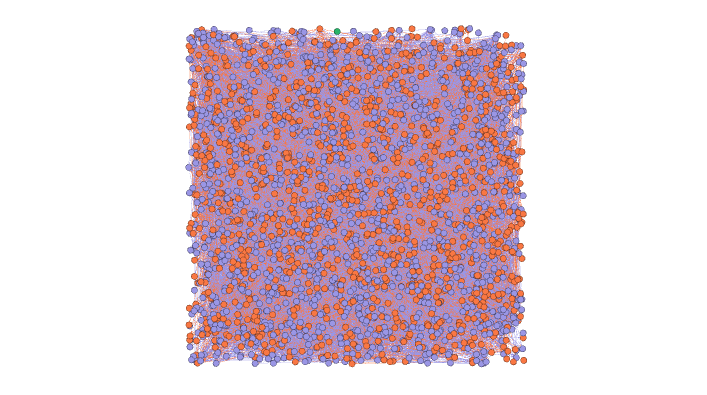
\includegraphics[height = 5cm]{pictures/Graph_without_layout.png}
    \caption{Полученный граф без укладки}
    \label{fig:graph_without_layout}
\end{figure}
Как видим на рисунке \ref{fig:graph_without_layout}, для получения легко читаемого графа необходимо <<раздвинуть>> вершины. Занимается этим различные алгоритмы укладки графа. Воспользуемся алгоритмом Фрюхтермана"=Рейнгольда, относящийся к семейству силовых алгоритмов,в котором используется пружинная физическая модель, где вершины определяются как тела системы, а ребра как пружины.
\begin{figure}[H]
\centering
    \begin{subfigure}[b]{0.3\textwidth}
        \centering
        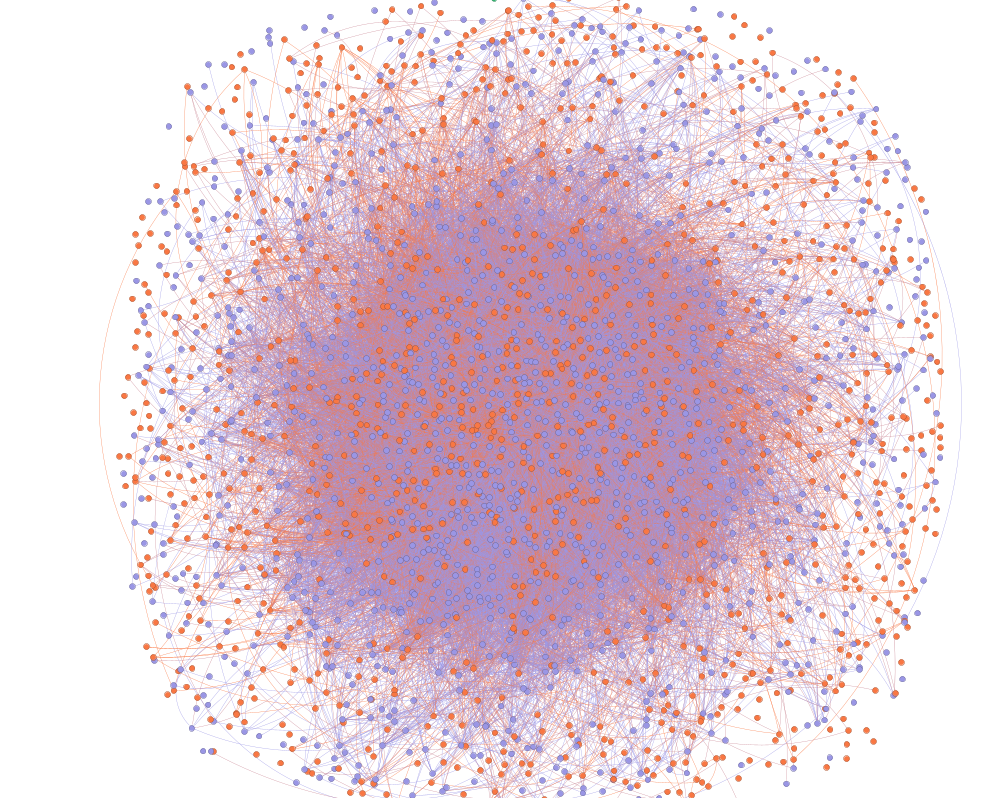
\includegraphics[width = \textwidth]{pictures/Layout_1.png}
    \end{subfigure}
    \begin{subfigure}[b]{0.3\textwidth}
        \centering
        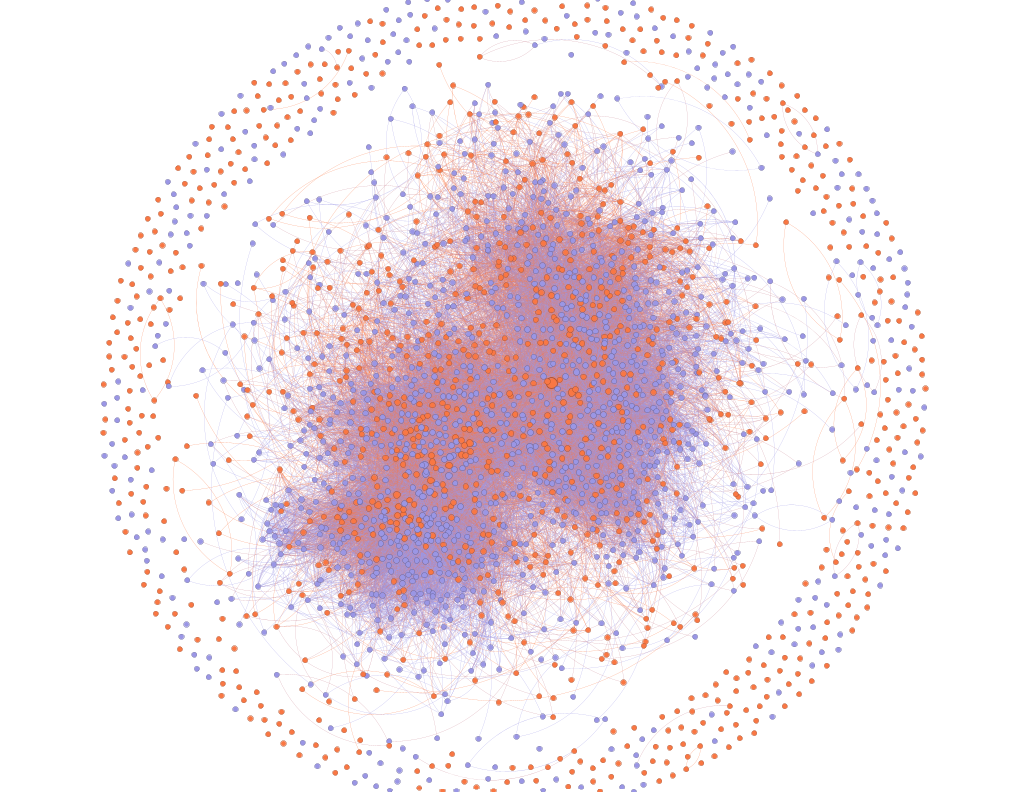
\includegraphics[width = \textwidth]{pictures/Layout_2.png}
    \end{subfigure}
    \begin{subfigure}[b]{0.3\textwidth}
        \centering
        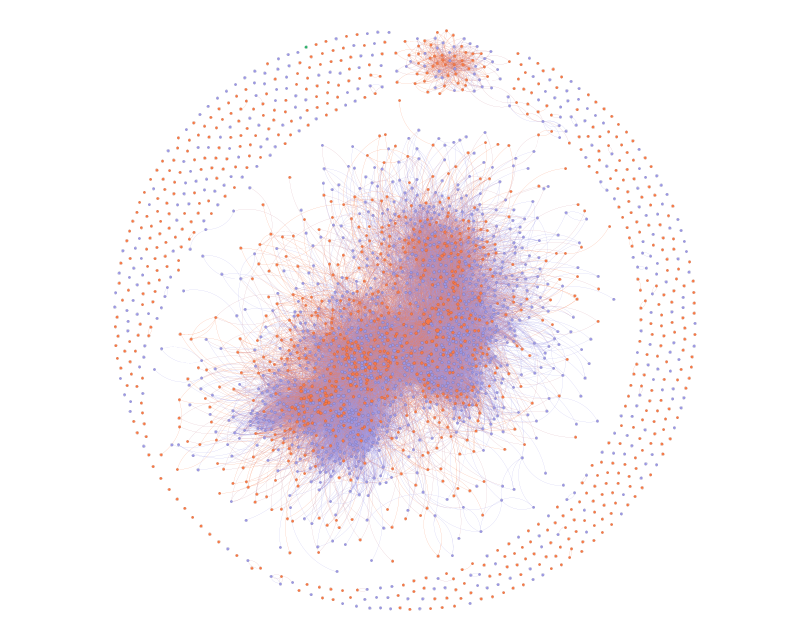
\includegraphics[width = \textwidth]{pictures/Layout_3.png}
    \end{subfigure}
    \caption{Процесс укладки графа}
    \label{fig:graph_layout}
\end{figure}

\begin{figure}[H]
    \centering
    \includesvg[height = 8cm]{pictures/Degree Centrality.svg}
    \caption{Полученный граф после укладки. Применена локальная центральность. Чем темнее вершина, тем больше у неё степень}
    \label{fig:graph_deg}
\end{figure}

Из рисунка \ref{fig:graph_deg} отметим темные вершины, именно они являются самыми общительными среди всех подписчиков.

Кроме того, заметим, что образовался круг из пользователей, который ни с кем не соединены. Вероятно они либо закрыли доступ к своим друзьям, либо являются ботами. Так же заметим, что образовался небольшой круг из пользователей, не связанных с центром. Анализируя эту группу, можно прийти к выводу, что все они являются жителями Санкт"=Петербурга.
% \begin{figure}[H]
%     \centering
%     \includesvg[height = 5cm]{pictures/Strongly component.svg}
%     \caption{Разбиене графа на компоненты сильной связности}
%     \label{fig:graph_strong_comp}
% \end{figure}

Применим к графу другие центральности:
\begin{figure}[H]
    \centering
    \begin{subfigure}[b]{0.45\textwidth}
        \centering
        \includesvg[width = \textwidth]{pictures/Clossenes Centrality.svg}
        \caption{Степень близости}
        \label{fig:graph_clossenes}
    \end{subfigure}
    \begin{subfigure}[b]{0.45\textwidth}
        \centering
        \includesvg[width = \textwidth]{pictures/Betweenes Centrality.svg}
        \caption{Степень посредничества}
        \label{fig:graph_betweenes}
    \end{subfigure}
    \caption{Применение к графу других центральностей}
    \label{fig:graph_centrality}
\end{figure}
Посмотрим на рисунок \ref{fig:graph_clossenes}. По нему можно сделать вывод, насколько человек близок к другим, то есть является ли он интровертом или экстравертом.

Обратимся теперь к графу на рисунке \ref{fig:graph_betweenes}, к которому применена степень посредничества. Она показывает, насколько много связей проходит через человека, то есть показывает, насколько он является незаменимым в данном графе.
% Раздел "Заключение"
\conclusion
В заключение, анализ социальных сетей является необходимым инструментом для понимания современного общества и его изменений. Благодаря этому инструменту можно выявлять тренды, понимать потребности и предпочтения людей, а также принимать обоснованные решения в бизнесе, политике и других областях деятельности. Перспективы развития анализа социальных сетей связаны с постоянным увеличением количества пользователей социальных сетей и их активности, а также с развитием технологий и методов анализа данных. В будущем, анализ социальных сетей будет играть еще более важную роль в понимании и прогнозировании поведения людей и общества в целом.
%Библиографический список, составленный вручную, без использования BibTeX
%
%\begin{thebibliography}{99}
%  \bibitem{Ione} Источник 1.
%  \bibitem{Itwo} Источник 2
%\end{thebibliography}

%Библиографический список, составленный с помощью BibTeX
%
%\nocite{*}
\inputencoding{cp1251}
\bibliographystyle{gost780uv}
\bibliography{thesis}
\inputencoding{utf8}

% % При использовании biblatex вместо bibtex
%\printbibliography

% Окончание основного документа и начало приложений
% Каждая последующая секция документа будет являться приложением
\appendix

\section{Исходный код на Python,осуществляющий сбор данных} 
\label{code}
\inputminted{python3}{../collect.py}


\end{document}